\subsection[Hist]{History}

\begin{frame}
  \frametitle{C/\cpp origins}
  \begin{minipage}{0.4\linewidth}
    \tikzstyle{old}=[ellipse,draw=black,fill=orange!30,thick,inner sep=2pt]
    \tikzstyle{new}=[rectangle,draw=black,fill=green!50,thick,inner sep=2pt]
    \tikzstyle{direct}=[<-,semithick]
    \tikzstyle{transverse}=[<-,dotted,semithick]
    \begin{tikzpicture}[->, node distance=.75cm, font=\tiny, scale=0.8, every node/.style={scale=0.8}]
      \node[old] (Simula)      {Simula};
      \node[left of=Simula,node distance=1.5cm] {1967};
      \node[old] (BCPL) [right of=Simula, node distance=2cm] {BCPL};
      \node[old] (B) [below of=BCPL] {B}
      edge[transverse] (BCPL);
      \node[old] (KandRC) [below of=B] {K and R C}
      edge[transverse] (B);
      \node[left of=KandRC,node distance=3.5cm] {1978};
      \node[old] (ClassicC) [below of=KandRC] {Classic C}
      edge[direct] (KandRC);
      \node[old] (CwithClasses) [below of=Simula,node distance=3cm] {C with Classes}
      edge[transverse] (Simula)
      edge[transverse] (BCPL)
      edge[direct] (ClassicC);
      \node[left of=CwithClasses,node distance=1.5cm] {1980};
      \node[old] (EarlyC++) [below of=CwithClasses] {Early \cpp}
      edge[direct] (CwithClasses);
      \node[left of=EarlyC++,node distance=1.5cm] {1985};
      \node[old] (C89) [below of=ClassicC,node distance=2.25cm] {C89}
      edge[direct] (ClassicC)
      edge[transverse] (CwithClasses);
      \node[old] (ARMC++) [below of=EarlyC++] {ARM \cpp}
      edge[direct] (EarlyC++)
      edge[transverse] (C89);
      \node[left of=ARMC++,node distance=1.5cm] {1989};
      \node[old] (C++98) [below of=ARMC++] {\cpp98}
      edge[direct] (ARMC++)
      edge[transverse] (C89);
      \node[old] (C99) [below of=C89] {C99}
      edge[direct] (C89)
      edge[transverse] (ARMC++);
      \node[left of=C++98,node distance=1.5cm] {1998};
      \node[new] (C++11) [below of=C++98] {\cpp11}
      edge[direct] (C++98)
      edge[transverse] (C99);
      \node[left of=C++11,node distance=1.5cm] {2011};
      \node[new] (C11) [below of=C99] {C11}
      edge[direct] (C99)
      edge[transverse] (C++98);
      \node[new] (C17) [below of=C11,node distance=1.8cm] {C17}
      edge[direct] (C11);
      \node[new] (C23) [below of=C17,node distance=1.2cm] {C23}
      edge[direct] (C17);
      \node[new] (C++14) [below of=C++11] {\cpp14}
      edge[direct] (C++11);
      \node[left of=C++14,node distance=1.5cm] {2014};
      \node[new] (C++17) [below of=C++14] {\cpp17}
      edge[direct] (C++14);
      \node[left of=C++17,node distance=1.5cm] {2017};
      \node[new] (C++20) [below of=C++17] {\cpp20}
      edge[direct] (C++17);
      \node[left of=C++20,node distance=1.5cm] {2020};
      \node[new] (C++23) [below of=C++20] {\cpp23}
      edge[direct] (C++20);
      \node[left of=C++23,node distance=1.5cm] {2023};
    \end{tikzpicture}
  \end{minipage}
  \begin{minipage}{0.57\linewidth}
    \begin{tabular}{cc}
      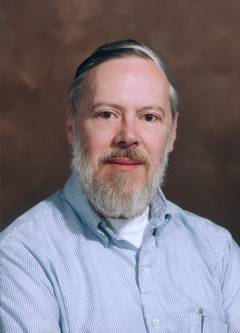
\includegraphics[height=2.5cm]{introduction/ritchie.jpeg} & 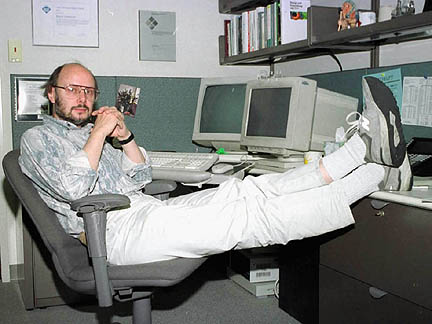
\includegraphics[height=2.5cm]{introduction/BjarneStroustrup.jpg} \\[-1ex]
      \tiny{C inventor} & \tiny{\cpp inventor} \\[-1ex]
      \scriptsize{Dennis M. Ritchie} & \scriptsize{Bjarne Stroustrup} \\
    \end{tabular}
    \begin{itemize}
      {\footnotesize
      \item Both C and \cpp are born in Bell Labs
      \item \cpp {\it almost} embeds C
      \item C and \cpp are still under development
      \item We will discuss all \cpp specs up to \cpp20 (only partially)
      \item Each slide will be marked with first spec introducing the feature
      }
    \end{itemize}
  \end{minipage}
\end{frame}

\begin{frame}
  \frametitle{\cpp11, \cpp14, \cpp17, \cpp20, \cpp23, \cpp26...}
  \begin{block}{status}
    \begin{itemize}
    \item A new \cpp specification every 3 years
      \begin{itemize}
      \item \cpp23 complete since 11th of Feb. 2023, awaiting ISO ballot
      \item work on \cpp26 has begun
      \end{itemize}
    \item Bringing each time a lot of goodies
    \end{itemize}
  \end{block}
  \pause
  \begin{block}{How to use \cpp XX features}
    \begin{multicols}{2}
      \begin{itemize}
      \item Use a compatible compiler
      \item add -std=c++xx to compilation flags
      \item e.g. -std=c++17
      \end{itemize}
      \vfill
      \columnbreak
      \begin{table}[h!]
        \begin{center}
          \begin{tabular}{c|c|c}
            \textbf{\cpp} & \textbf{gcc} & \textbf{clang}\\
            \hline
            11 & $\geq$4.8 & $\geq$3.3\\
            14 & $\geq$4.9 & $\geq$3.4\\
            17 & $\geq$7.3 & $\geq$5\\
            20 & $>$11  & $>$12 \\
          \end{tabular}
          \caption{Minimum versions of gcc and clang for a given \cpp version}
        \end{center}
      \end{table}
    \end{multicols}
  \end{block}
\end{frame}
